\chapter{Funkcja celu -- porównanie barwy dźwięku}~\label{target_function_chapter}

Aby stopniowo dostosować graf przetwarzania sygnałów zaimplementowany 
w rozdziale~\ref{dsp_graph_chapter} do imitowania zadanej próbki dźwięku,
należy wykorzystać funkcję celu, która maleje wraz ze wzrostem podobieństwa
barwy dźwięku między próbki zadaną i sygnałem generowanym przez graf. 

\begin{figure}[H]\label{fig:waveform_not_equal_to_perception}
    \centering
    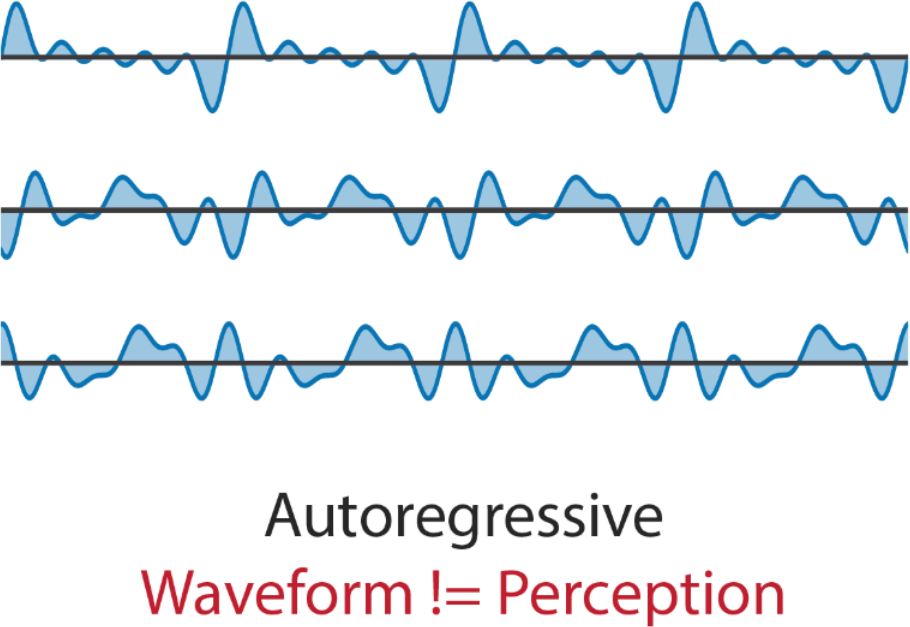
\includegraphics[width=0.5\linewidth]{rys03/d_dsp_example_graph.png}
    \caption{
      Przykład trzech próbek dźwięku, które dla słuchacza brzmią identycznie, mimo
      znacznych różnic w kształcie fali. Źródło obrazka:~\cite{engel2020ddsp}.
    }
\end{figure}

\section{Porównanie barwy dźwięku w literaturze}\label{sec:timbre_comparison_literature_overview}

Żadna z prac przeanalizowanych podczas przeglądu literatury
(\cite{engel2020ddsp},~\cite{ieee_synth_programming},~\cite{ddx7},~\cite{riffusion},~\cite{evolutionary_puredata},~\cite{parallel_evolutionary_optimization_synth_parameters},~\cite{mfcc_dtw})
nie wykorzystuje metod porównywania sygnału osadzonych jedynie w dziedzinie czasu, ponieważ
nie są one skuteczne do porównywania dźwięków pod względem odczuć psychoakustycznych.
Przykład różnych kształtów fali, które z perspektywy słuchacza brzmią jak
taki sam dźwięk zademonstrowano na rysunku~\ref{fig:waveform_not_equal_to_perception}.

Ponieważ porównywanie barwy dźwięku instrumentów muzycznych nie należy do popularnych
tematów badań, podczas przeglądu literatury wykorzystano również badania dotyczące
rozpoznawania głosu, wykorzystujące współczynniki MFCC oraz
\textit{dynamic time warping}~(DTW)~\cite{mfcc_dtw}.

\subsection{Systematyzacja metod z literatury}~\label{sec:timbre_comparison_systematisation}

Metody zaczerpięte z literatury wykorzystują różne podejścia do porównywania barwy dźwięku
pomiędzy sygnałami. Podejścia te można usystematyzować za pomocą dwóch cech:

\begin{enumerate}
  \item Rodzaj wykonanej transformacji do dziedziny częstotliwości:
  \begin{itemize}
    \item transformata Fouriera (w różnych konfiguracjach)~\cite{riffusion}~\cite{ddx7},
    \item MFCC~\cite{ieee_synth_programming}~\cite{evolutionary_puredata}~\cite{mfcc_dtw}.
  \end{itemize}
  \item Dalsze przetwarzanie przetransformowanego sygnału w celu ułatwienia optymalizacji:
    \begin{itemize}
      \item dostosowywanie wagi konkretnych próbek na podstawie metryki określającej siłę sygnału
        (na przykład \textit{root-mean-square}, RMS)~\cite{parallel_evolutionary_optimization_synth_parameters},
        aby wzmocnić istotność głośniejszych fragmentów dźwięku,
      \item wykorzystanie \textit{dynamic time warping}, aby funkcja celu przyzwalała na
        niedokładności w odwzorowaniu dokładnej dynamiki zmian w charakterystyce spektralnej~\cite{mfcc_dtw}.
    \end{itemize}
\end{enumerate}

\subsection{Wybór funkcji celu do przetestowania}

Na podstawie analizy metod z literatury opisanej w rozdziale~\ref{sec:timbre_comparison_systematisation} zostały wybrane wszystkie warianty
funkcji celu wykorzystywane w przeanalizowanej literaturze:

\begin{enumerate}
  \item Różnica w spektrum Fouriera,
  \item Różnica w spektrum Fouriera liczona za pomocą DTW,
  \item Różnica w MFCC,
  \item Różnica w MFCC liczona za pomocą DTW\@,
  \item Różnica w MFCC ważonym za pomocą RMS\@.
\end{enumerate}

\section{Proces testowania funkcji celu}

\begin{figure}[H]\label{fig:fm_graph_for_benchmarks}
    \centering
    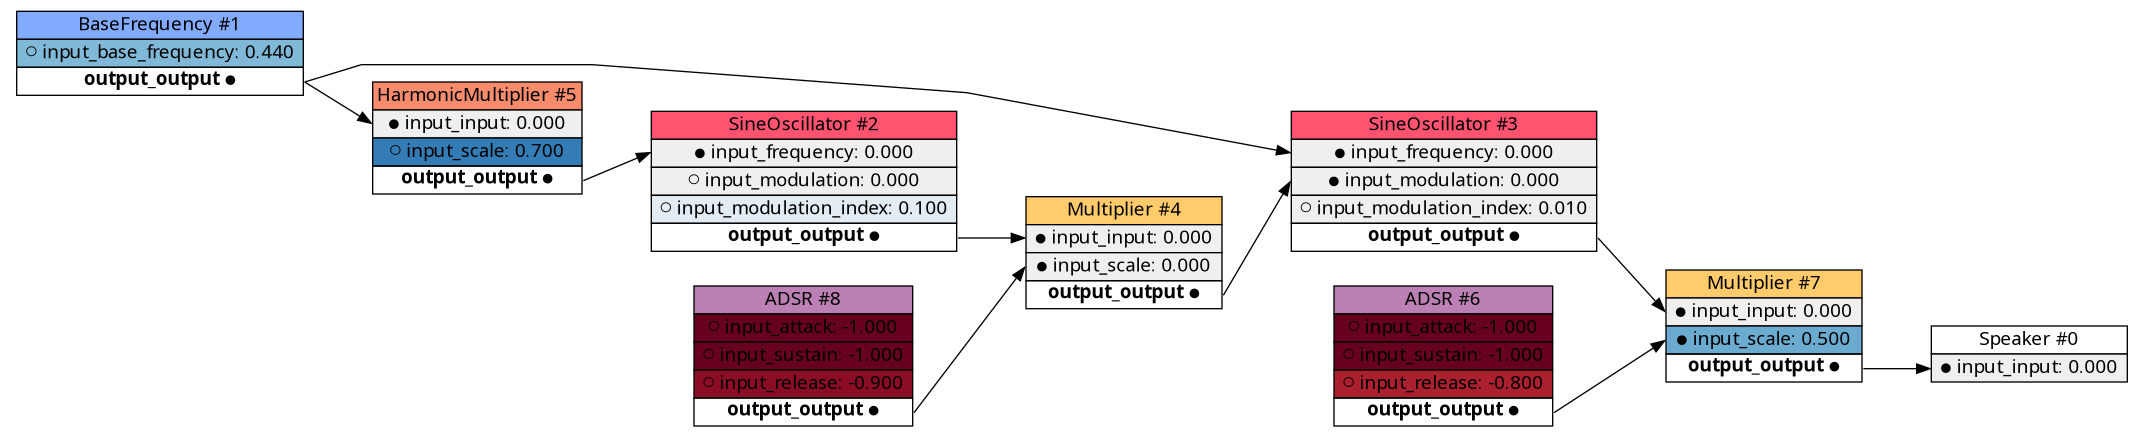
\includegraphics[width=1.0\linewidth]{rys03/fm_graph_for_benchmarks.png}
    \caption{
      Prosty graf syntezy FM, zawierający jeden oscylator służący za sygnał nośny
      i jeden oscylator służący za sygnał modulujący.
    }
\end{figure}

Funkcje celu zostały przetestowane poprzez wykonanie
zbioru przekrojów przez uproszczony problem syntezy typu FM oraz
przez przeprowadzenie próby dostosowania parametrów dwóch grafów
o predefiniowanej strukturze, dla syntezy FM oraz \textit{analog modeling}.

\section{Przekrój wartości funkcji celu dla prostego problemu syntezy typu FM}

Testy obejmowały wygenerowanie wartości funkcji celu podczas
modyfikowania pojedynczego parametru w grafie przetwarzania sygnałów
przedstawionym na rysunku~\ref{fig:fm_graph_for_benchmarks}.
Modyfikowane parametry odpowiadają za różne cechy barwy uzyskanego dźwięku:

\begin{itemize}
  \item \texttt{HarmonicMultiplier/input\_scale}: częstotliwość modulacji FM,
  \item \texttt{SineOscillator/input\_modulation\_index}: siła składowych harmonicznych,
  \item \texttt{ADSR/input\_attack}: dynamika dźwięku.
\end{itemize}


\begin{figure}[H]\label{fig:target_function_testing}
    \centering
    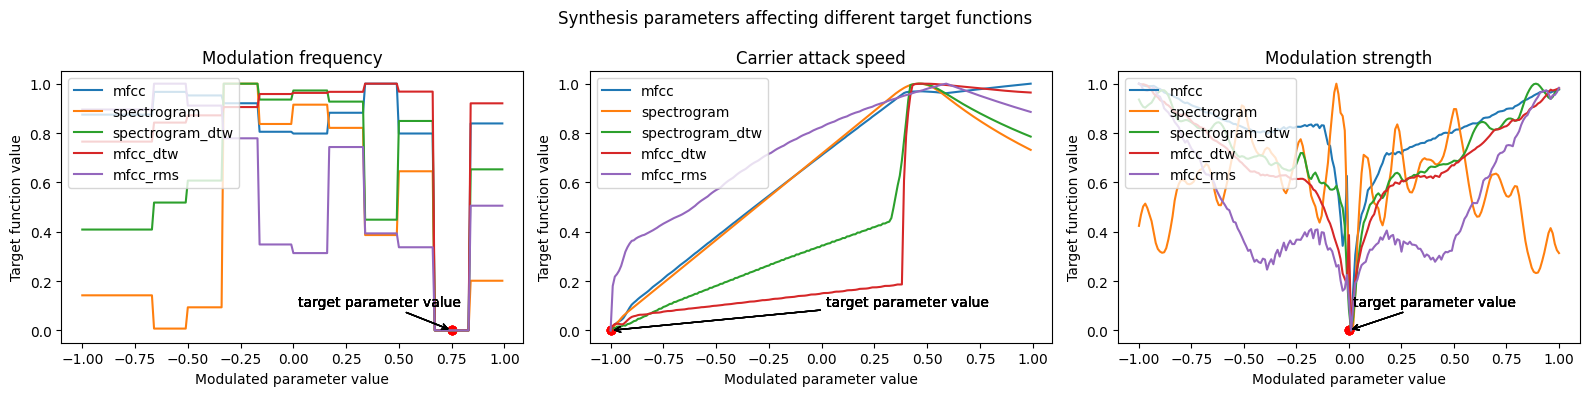
\includegraphics[width=1.0\linewidth]{rys03/target_function_testing.png}
    \caption{
      Zmiany w wartościach testowanych funkcji celu podczas przesuwania różnych parametrów syntezy dźwięku. 
      Kształt pierwszego wykresu wynika z zastosowania kwantyzacji dostępnych częstotliwości modulacji,
      aby wykluczyć nieharmoniczne stosunki częstotliwości modulacji i nośnej. Tego rodzaju praktyka
      jest wykorzystywana w syntezatorach FM~\cite{digitone_manual}, ponieważ ułatwia dostosowywanie parametrów syntezy.
    }
\end{figure}

\subsection{Analiza wyników}

Wyniki testów zaprezentowane na wykresach~\ref{fig:target_function_testing} pozwalają na
wyeliminowanie bezpośredniej różnicy między spektrogramami jako funkcji celu,
ponieważ w przypadku zmian częstotliwości modulacji posiada ona minimum globalne w 
niewłaściwej pozycji parametru.

\subsubsection{Częstotliwość modulacji FM}

Wszystkie funkcje z wyjątkiem różnicy między spektrogramami pokazują poprawną, 
najniższą wartość dla właściwej wartości parametru.

\subsubsection{Dynamika dźwięku}

W przypadku wpływu zmian w dynamice dźwięku na wartości funkcji celu,
zastosowanie DTW znacząco zmienia kształt funkcji celu, zależnie od wybranego rozmiaru
okna DTW\@. Duży rozmiar okna powoduje zmniejszenie kary za niedokładne odwzorowanie
dynamiki dźwięku. 

\subsubsection{Siła modulacji}

Różnica między spektrogramami jest najbardziej chaotyczna, nie maleje wraz
ze zbliżaniem się do poprawnej wartości parametru. Pozostałe funkcje celu
wykorzystujące \textit{MFCC} mają lepszą charakterystykę -- maleją
wraz ze zbliżaniem się do poprawnej wartości parametru.

\section{Optymalizacja parametrów dla predefiniowanych
grafów syntezy FM oraz \textit{analog modeling}}

% \begin{enumerate}
%   \item Zastosowanie DTW może pogorszyć 
% \end{enumerate}

